%Präambel
\documentclass[a4paper,12pt]{scrartcl}
\usepackage[utf8]{inputenc}
\usepackage[T1]{fontenc}
\usepackage{ngerman, graphicx}

%Seite einrichten
\areaset[2cm]%               % Zusätzlicher Rand für die Bindung
        {17cm}{24cm}         % Textbreite und -Höhe
        
%Zeilenabstand/-vorschub, statt parskip
\renewcommand{\baselinestretch}{1.24}

%Linienstärke
\newcommand\HRule{\noindent\rule{\linewidth}{1.5pt}}

\begin{document}

%Titelblatt
\begin{titlepage}

\begin{minipage}[c]{5cm}
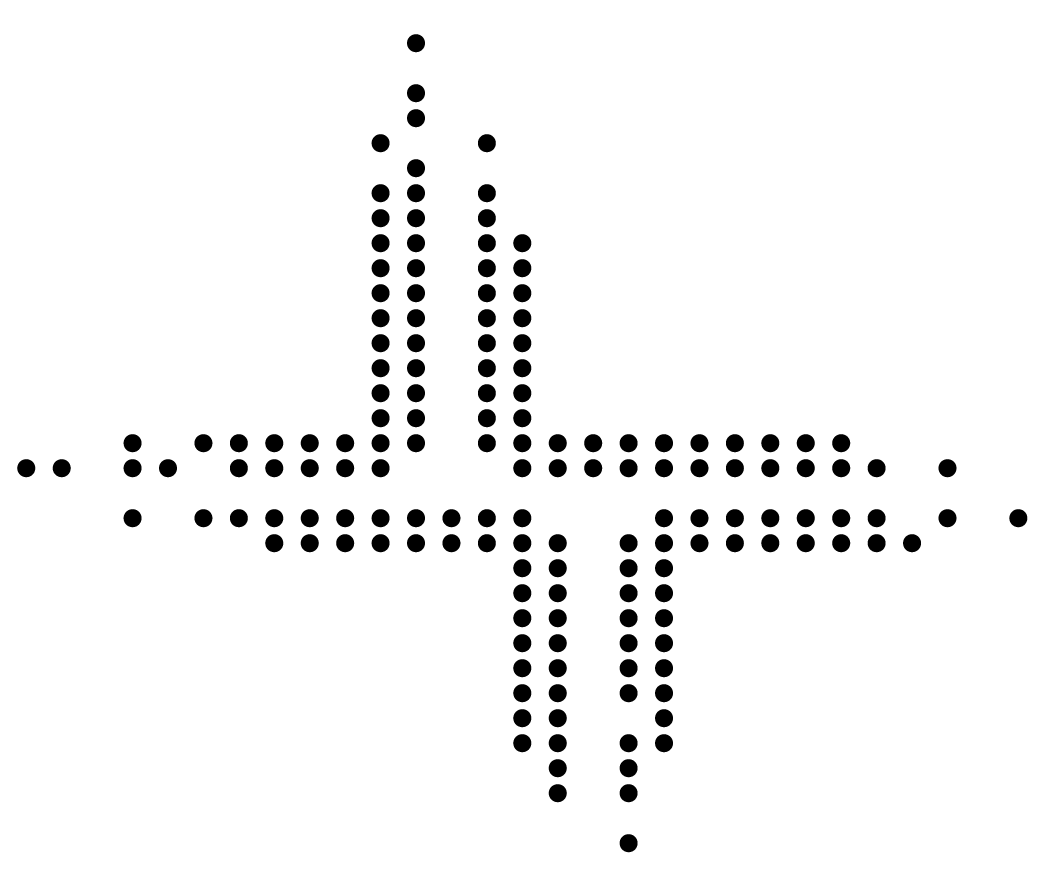
\includegraphics[width=5cm]{logohdafbi-standalone}
\end{minipage}
\hfil
\begin{minipage}[c]{10cm}
\begin{flushright}
\Large Einführung in die Technik\\und Anwendung von\\
\LARGE \textbf{RFID}
\end{flushright}
\end{minipage}

\vspace*{1cm}

\begin{minipage}[c]{8cm}
\begin{flushleft}
\large David Falk (736532)\\Christian Lichtsinn (736787)\\Praktikum 1 \& 2: 19.10.15 \& 02.11.15
\end{flushleft}
\end{minipage}
\hfil
\begin{minipage}[c]{8cm}
\begin{flushright}
\large Betreuer:\\Prof. Ralf S. Mayer\\F. Dotzauer, E. Wagner
\end{flushright}
\end{minipage}

\vspace*{1cm}

\HRule

\vspace*{\stretch{1}}

\centering
\huge

\begin{bfseries}
AutoID

Resonanz

Frequenzen

RFID-Grundlagen
\end{bfseries}

\vspace*{\stretch{1}}

\end{titlepage}
\pagenumbering{arabic} %Setzt hier die Seite auf '1' zurück, Titel ist 'seitenlos'

%ab hier normal weiter
\section{OCR}
\section{Barcodes}
\subsection{Welche Arten von Barcodes kann das Gerät erfassen?}
\begin{itemize}
  \item EAN 8
\end{itemize}
\subsection{Wie viele Barcodes können in einer bestimmten Zeit erfasst werden?}
\subsection{Wie ändert sich die Erkennung mit Abstand, Winkel, Abdeckung, Einfluss von Licht?}
\subsection{Welche Auswirkung hätte Verschmutzung, Beschädigung des Barcodes?}
\subsection{Hängt die Lesegeschwindigkeit mit der Informationsmenge im Code zusammen?}

\section{Oszilloskop, Spektrumanalysator und Frequenzgenerator}

\section{Schwingkreis, Resonanz, Lastmodulation und -Demodulation}

\section{1,3GHz Mikrowellen}

\section{RFID HF}

\section{NFC}
\subsection{Was ist NFC?}
NFC ist eine Art RFID, bei der die stikte Trennung zwischen Lesegerät und Tag/Transponder aufgehoben wird.
NFC verwendet den HF-Bereich bei 13,56 MHz.
\subsection{Vorbereitete Tags}
\subsection{Tag konfigurieren}
\subsection{Übertragung zwischen zwei Smartphones}
Mit Android Beam ist es möglich Inhalte zwischen zwei Android-Telefonen übertragen.
Wir konnten eine URL übertragen, wenn eine Website geöffnet ist und den App Store
öffnen, wenn eine App geöffnet ist.

\end{document}